\documentclass[12pt]{article}
\usepackage{graphicx}
\usepackage{amsmath}
\usepackage{subcaption}

%opening
\title{CSCI 491, Project P3\\
		\small{Data Visualization Figures}}
\author{Group 8\\
		\small{Tao Huang and James Soddy}}

\begin{document}

\maketitle

For our project, we are investigating the shape of play by various poker players. We have
met with some difficulty in finding usable ways to represent our data. We have some visualizations,
though, which help to illustrate both the promise of our approach as well as the difficulties we
are facing. Our first figures give some shape to our expectation of how the data should look,
and we then use plots of two different players' data for comparison and contrast.

\newpage
\section*{Establishing a baseline}

As we started visualizing our data, we realized that it would be useful to have both an
expectation of what the data should look like, and a measure against which some aspects of
the data can be considered. In poker, an obvious analysis of a player's style is to
inspect the different ways in which they play hands with different values. With that in mind, we
created these plots, which show the actual value of two-card starting hands when played in
Texas Hold'Em poker. We thought that the more similarity between the shape of these figures
and the shape of an individual player, the more rationally that player was playing.

\begin{figure}[ht!]
	\makebox[\linewidth][c]{%
	\begin{subfigure}[b]{0.6\textwidth}
		\centering
		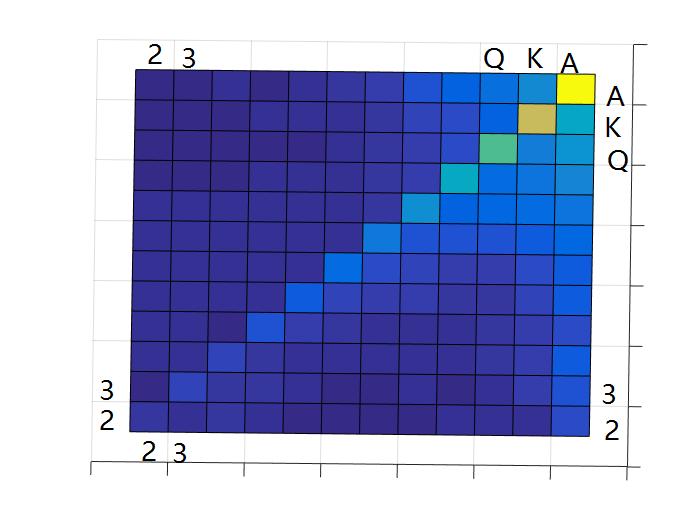
\includegraphics[width=.95\textwidth]{score}
  		\caption{\textbf{Heatmap of Poker Hand Values.} All possible differently valued staring Hold'Em
  		hand combinations aligned in a grid, with their color indicating profitability}
  	\end{subfigure}
  	\begin{subfigure}[b]{0.6\textwidth}
  		\centering
		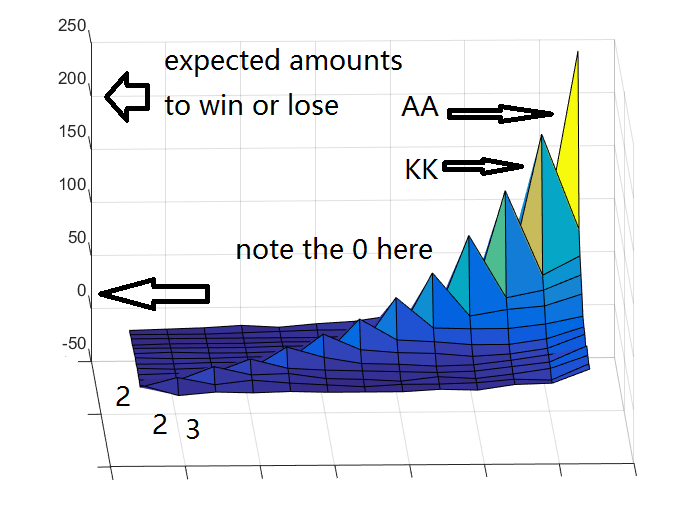
\includegraphics[width=.95\textwidth]{score1}
		\caption{\textbf{Poker Hand Values Elevation.} The same data, showed as an elevation plot
		so that the different hand values become clear. The Z-axis is in big-blinds.}
	\end{subfigure}
	}\\
\end{figure}

\newpage

\section*{Player A}

We broke player data into two random groupings, and plotted it in the same way as the hand
value data in the figures above. This time, rather than the value of the hands, we plotted the
amount of money the players were willing to invest in order to play the hands. Similarities
between these figures and our baseline figures are obvious, but so are differences between all
of them, as well as artifacts of our data.

\begin{figure}[ht!]
	\makebox[\linewidth][c]{%
	\begin{subfigure}[b]{0.6\textwidth}
		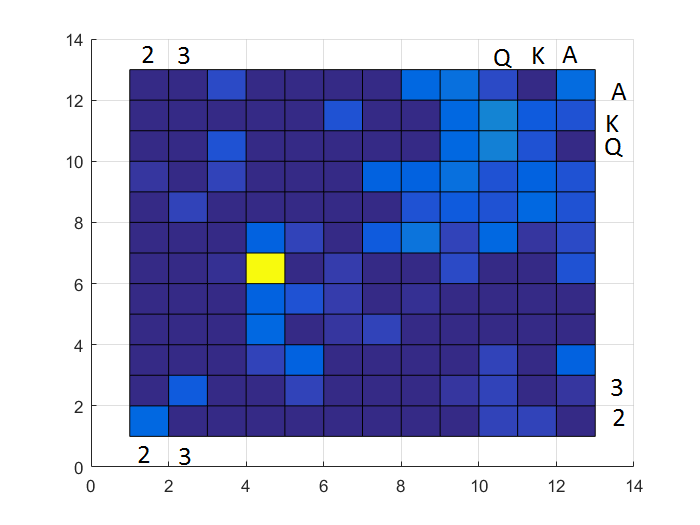
\includegraphics[width=.95\textwidth]{A0mR}
  		\caption{\textbf{Sample A Heatmap.} The shape from above is recognizable, though quite 
  		distorted.}
  	\end{subfigure}
  	\begin{subfigure}[b]{0.6\textwidth}
		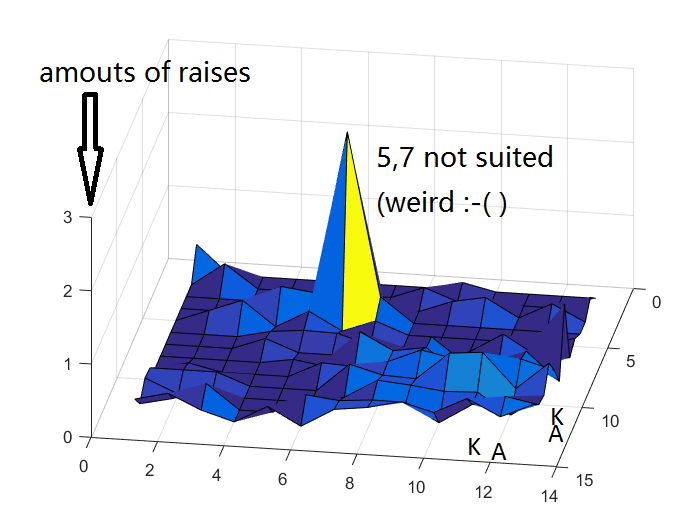
\includegraphics[width=.95\textwidth]{A0mR1}
  		\caption{\textbf{Sample A Elevation.} The huge outlier is an artifact of too little 
  		usable data.}
	\end{subfigure}
	}\\
	\makebox[\linewidth][c]{%
	\begin{subfigure}[b]{0.6\textwidth}
		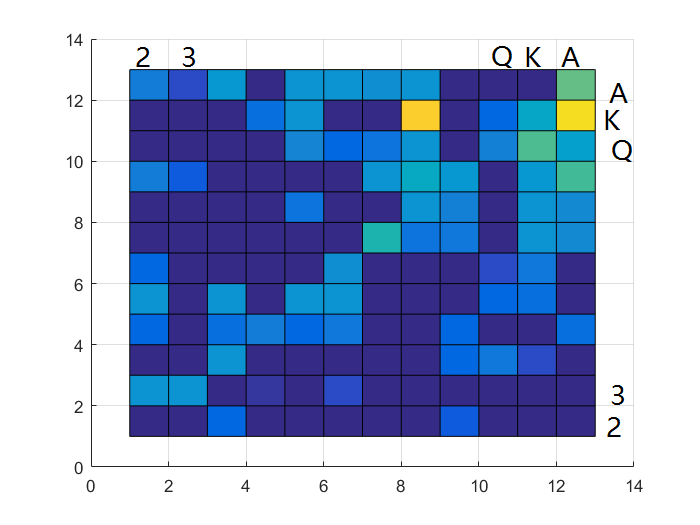
\includegraphics[width=.95\textwidth]{B0mR}
  		\caption{\textbf{Sample B Heatmap.} Fortunately, this looks fairly similar to the
  		first Player A sample.}
  	\end{subfigure}
  	\begin{subfigure}[b]{0.6\textwidth}
		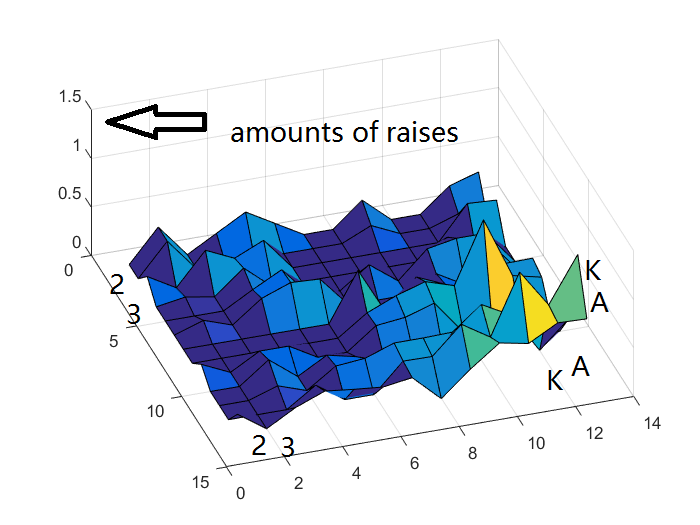
\includegraphics[width=.95\textwidth]{B0mR1}
  		\caption{\textbf{Sample B Elevation.} Variation due to the limited available data is
  		our limiting factor.}
	\end{subfigure}
	}\\
\end{figure}

\newpage


\section*{Player B}

Another player's data represented in figures. This data illustrates that our methods are not
quite ready. These two samples from one player are more different from each other than any
of our other figures. However, the uniform height of the peaks on both samples give hope
that improved datasets might clean up our results significantly.

\begin{figure}[ht!]
	\makebox[\linewidth][c]{%
	\begin{subfigure}[b]{0.6\textwidth}
		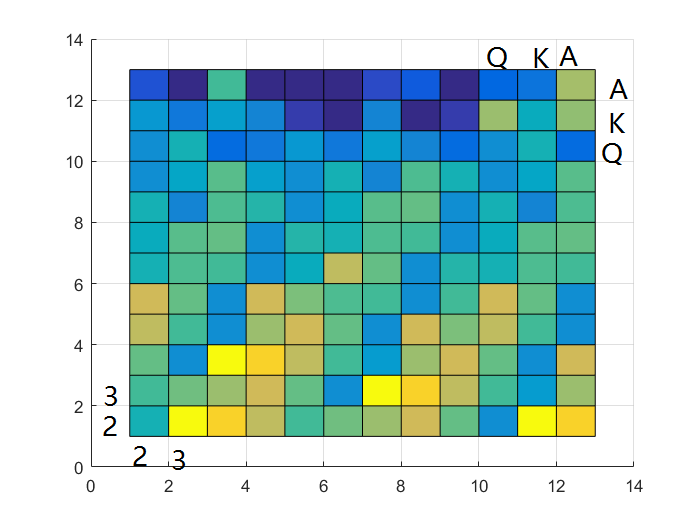
\includegraphics[width=.95\textwidth]{AEL5}
  		\caption{\textbf{Sample A Heatmap.} This bears no resemblance to the hand value figure.}
  	\end{subfigure}
  	\begin{subfigure}[b]{0.6\textwidth}
		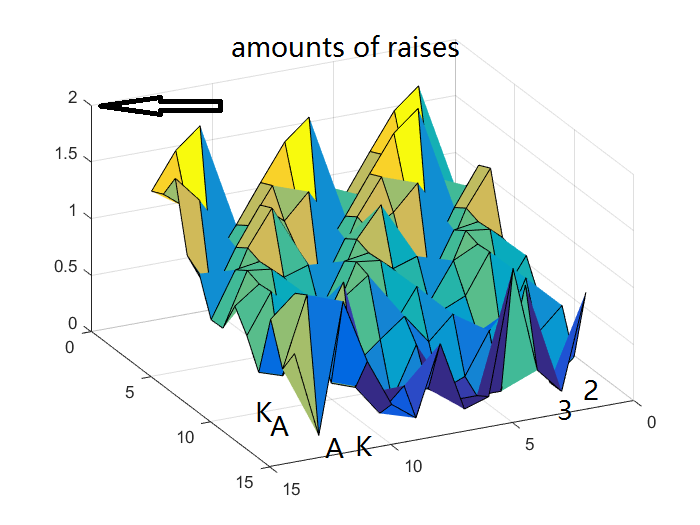
\includegraphics[width=.95\textwidth]{AEL51}
  		\caption{\textbf{Sample A Elevation.} Not only is the diagonal ridge gone, but there is
  		very little height variation.}
	\end{subfigure}
	}\\
	\makebox[\linewidth][c]{%
	\begin{subfigure}[b]{0.6\textwidth}
		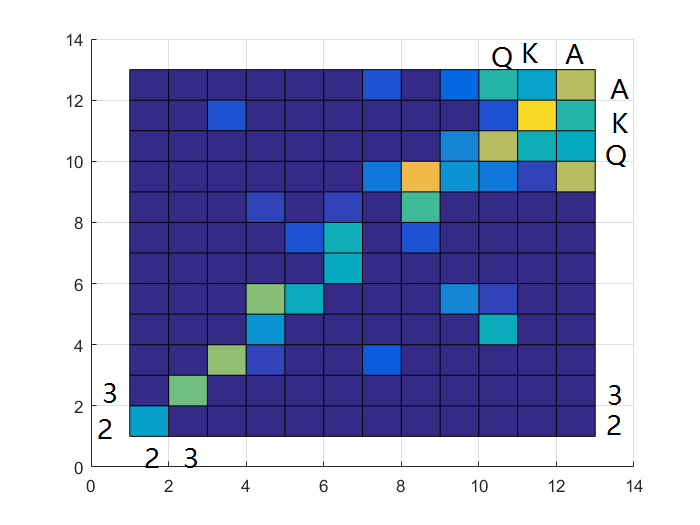
\includegraphics[width=.95\textwidth]{BEL5}
  		\caption{\textbf{Sample B Heatmap.} This figure is unfortunately quite different from
  		Sample A.}
  	\end{subfigure}
  	\begin{subfigure}[b]{0.6\textwidth}
		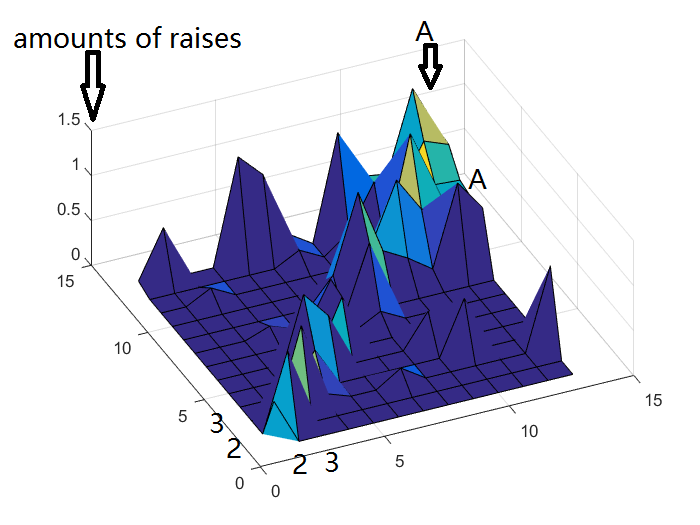
\includegraphics[width=.95\textwidth]{BEL51}
  		\caption{\textbf{Sample B Elevation.} The peaks on this figure are still fairly uniform in
  		height.}
	\end{subfigure}
	}\\
\end{figure}


\newpage

\section*{In Conclusion}

In spite of the millions of hands of data which we have access to, and the fact that there are
tens of thousands of hands available for some players, our data samples are not sufficient for
the types of analysis we are attempting. There are two main issues at hand here. The first is
that the inherent randomness of poker means that many types of situations only come up very
rarely, so data about them converge very slowly. So slowly in fact that it is probable that what
is being measured will have changed before sufficient data are collected to measure it. The second
problem is that most of our hand histories do not tell us what the players' hole cards are. Even
for some players with many thousands of hands, we have fewer than 1000 hands with card information.
With 144 different starting hand possibilities, that just isn't enough repeats of each hand
to smooth out variation in play, which makes our distance calculations suspect.

Just to achieve figures as meaningful as the ones presented here, we have had to simplify
our approach to just two cards and the first round of betting. Unfortunately, this excludes
most of the human interaction which is the key aspect of interest in poker and other games.
In order to bring more interaction into our analysis, we need to find some way to smooth out our
initial steps considerably. Our results on this early data are already suspect, and we think
it would be too much to ask of our data to yield to deeper probing of human interaction.

That is why we think these figures we have chosen are suitable to represent both the promise of,
and the problems with, our project so far.



 
        
  
 

\end{document}